\section{TGFB superfamily signaling}
\label{pathways:tgfb}

\subsection{Brief overview of the \tgfbsf\ signaling network}

\tgfbsf\ represents a broad array of morphogenic signals \cite{Schmierer2007} 
that are deeply conserved across the metazoa.
Orthologs of each pathway component are found in nematodes,
flies, mammals,
and even the basal metazoan \textit{Trichoplax adhaerens}
\cite{VonBubnoff2001,Srivastava2008,Huminiecki2009}.
These pathways are functionally essential to organismal development and
adult tissue homeostasis, and are therefore frequently mis-regulated
in cancer and other pathologies. Despite their general importance, activity of
these pathways yields broad context-dependency in phenotypic outcomes 
\cite{Massague1990,Massague2000,VonBubnoff2001,Wagner2007,Schmierer2007,
Umulis2009,Massague2012}.


The network structure of the canonical \tgfbsf\ pathway is simple
enough to prompt the statement that it has been ``solved, to a first 
approximation \cite{Massague2012}.'' It includes only three primary
nodes: homodimeric ligands \arp{pathways:tgfb:ligands}
that bind to heterodimeric receptors \arp{pathways:tgfb:receptors}
which, in turn, activate the downstream Smad family of
transcription factors
\arp{pathways:tgfb:smads}. Figure \ref{fig:pathways:tgfb} shows the
structure of the \tgfbsf\ pathway and the diversity of its components
as discussed below.


Throughout this section, it is important to be aware that
the degree of functional overlap between the various TGFB superfamily
members is poorly established. Most studies of these pathways include
only one or a few families at a time and, likely due to historical reasons, each family
has been primarily studied in the context of a handful of tissues or
diseases. Therefore, having a function ascribed to one \tgfbsf\
member does not at all imply that other members do not have that function.
For this reason I often refer to the superfamily in general even
for functions that are known only to a subset of its members.


  \begin{figure}[!bt]
  \centering
  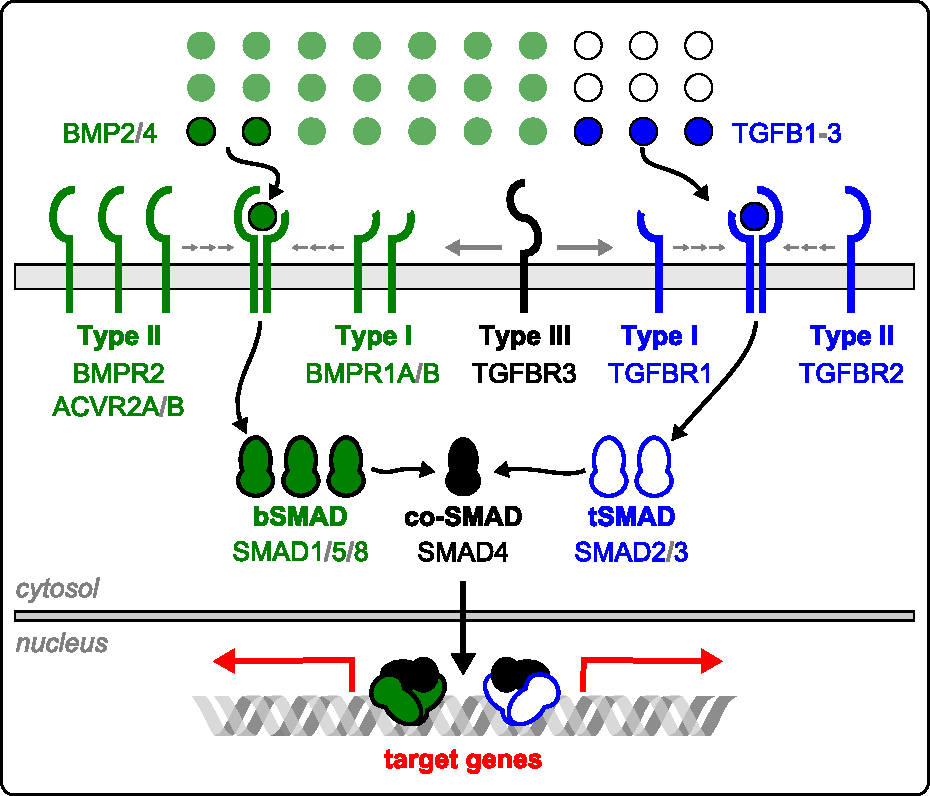
\includegraphics[width=4in]{FIGS/pathways/tgfb.pdf}
  {\singlespacing 
  \caption[Structure of the \tgfbsf\ signaling pathway]
        { Structure of the \tgfbsf\ signaling pathway.
          $\sim$30 homodimer ligands (circles) are classified into
          $\sim$20 BMPs (green), 3 \tgf s (blue), and others (outlines).
          BMP2/4 and \tgf 1-3 have distinct sets of receptors. Upon ligand
          binding, Type II receptors activate Type I receptors. In turn, active
          Type I receptors phosphorylate downstream Smads, specifically the \tgf-rSmads
		  (tSmads) or the BMP-rSmads (bSmads) (see \ar{pathways:tgfb:smads}).
		  Upon \pn\ the rSmads associate with Smad4,
          translocate to the nucleus, and bind promoters to affect transcription.
  }
  \label{fig:pathways:tgfb}}
  \end{figure}




\subsection{The \tgfbsf\ ligands}
\label{pathways:tgfb:ligands}

The more than thirty diverse ligands of the TGFB
superfamily are spread across several families,
each having a different degree of homology within their ranks
\cite{Massague2005,Ehrlich2011,Wakefield2013}. The families
include three prototypical \tgf s and
over twenty Bone Morphogenic Proteins (BMPs), as well as various Activins, Inhibins,
Growth/differentiation Factors (GDFs) and others
\cite{Massague1990,Miyazono2005,Schmierer2007}
(see the phylogenetic tree in \ar{fig:tgfb:trees}).
In this review I focus on the \tgf s and BMPs. These two families are
well-studied in the context of mammalian development and
disease and, as I describe below, they are selective for distinct receptors as well as
downstream transcription factors.


\tgfbsf\ ligands are initially made as large precursor proteins.
These precursors are cleaved intracellularly,
allowing the non-ligand portion of the precursor, the so-called
``Latency-associated peptide (LAP),'' to remain
non-covalently associated \cite{Khalil1999}. This interaction is inhibitory
and so the resulting inactive complex 
is secreted into the extracellular space.
Within this non-signaling complex resides the mature homodimeric
\tgfbsf\ ligand.


Within the mature ligand dimer, each
monomer forms a ``cysteine knot'' composed of internal
di-sulfide bridges between three cysteine-cysteine pairs.
The two monomers are covalently linked by an additional intramolecular
cysteine-cysteine bridge \cite{Nohe2004,Schmierer2007}.
The active homodimer is revealed, and then able to bind to its receptors, by separation
from the inhibitory complex. Experimentally, this
separation can be induced by various
conditions (e.g. low pH or the addition of chaotropic salts or certain proteases).
In cells, the evidence suggests that
separation is a mechanical process performed by integrins
\cite{Massague1990,Khalil1999,Shi2011}.


The three prototypical \tgf s are highly homologous,
though they have small differences in their
tertiary structures that allow for some divergence in affinities for binding partners.
\cite{Robertson2013}. For example, \tgf 2 requires a co-receptor for binding to
its cognate receptors, while \tgf 1/3 do not.
Despite these differences, the functions of the
three \tgf s are thought to be essentially the same. Therefore,
their effects in cells are expected to be a property of
\i{where} and \i{when} a member
is expressed, not \i{which} is expressed \cite{Radaev2010}.
In my own experiments, I find that
\tgf 1 and \tgf 3 do indeed produce the same phenotypic effects,
though I
observe $\sim$10-fold differences in potency between these two ligands
(data not shown).


The BMPs show a much larger degree of evolutionary diversity
than do the \tgf s, and can be broken into several
subfamilies by both homology and function (see \ar{fig:tgfb:trees}). The BMPs have
differential specificity to several receptors, and have relatively
low receptor affinity in comparison to the \tgf s (nanomolar
versus picomolar \cite{Ehrlich2011}). Along with tissue-specific 
expression patterns, this differential affinity
may account for the putative functional specificities attributed
to each BMP. Further, there are a large number of extracellular
secreted proteins that can differentially antagonize BMP signaling
(e.g. Noggin, Chordin, Gremlin, and Cerberus).


The differential receptor- and antagonist-binding affinities of
the BMPs are frequently cited as responsible for the idiosyncratic signaling outcomes
across this ligand family \cite{VonBubnoff2001,Zakin2010}. Importantly,
this is suggestive that each of these ligands may then carry the same
information. The context-dependency
may then simply stem from differences in the effective concentrations of the ligands.
There is evidence for this, since there is 
broad functional redundancy across the entire BMP family.
For example, knockout experiments in mice show that ablation of individual BMPs yields
developmental defects but only rarely lethality (BMP2/4 being the notable
exceptions) \cite{Sieber2009,Bandyopadhyay2013}. 


For simplicity, in the rest of this dissertation I focus on only one of the
BMP subfamilies. This family is composed of
BMP2 and BMP4, orthologs of \fly\ Decapentaplegic (DPP) \cite{Miyazono2005}.
This family is
highly studied in the context of mammalian stem cell differentiation and reperesents
a distinct information channel from the \tgf\ family also studied in this dissertation
(i.e. the receptors and downstream effectors are mostly non-overlapping) .


  \begin{figure}[!bt]
  \centering
  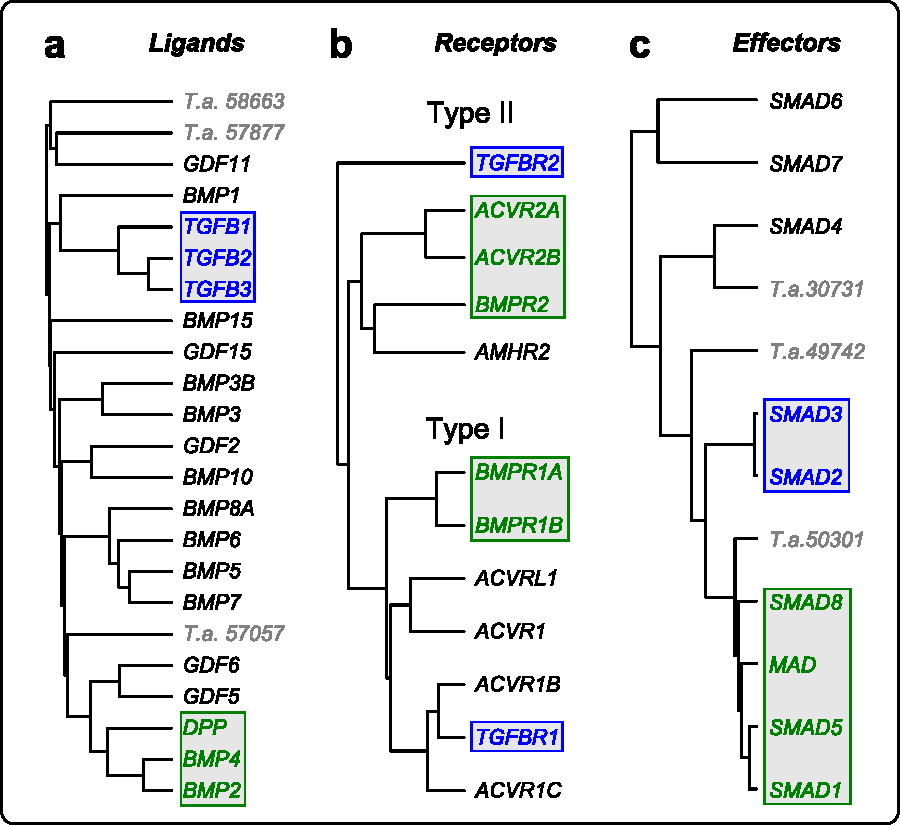
\includegraphics[width=4in]{FIGS/pathways/tgfb_tree.pdf}
  {\singlespacing 
  \caption[\tgfbsf\ phylogenetic trees]
            { Phylogeny of the \tgf\ and BMP pathway
              ligands  (\textbf{a}, \autoref{pathways:tgfb:ligands}),
              receptors (\textbf{b}, \autoref{pathways:tgfb:receptors}), and
              transcription factors (\textbf{c}, \autoref{pathways:tgfb:smads}).
              The \textit{T.a.} prefix indicates putative \ta\ proteins (gray).
			  DPP and MAD are \fly\ orthologs of BMP2/4 and Smad1/5/8.
              \tgf-specific nodes (blue) and BMP2/4-specific nodes (green) are highlighted.
              See \cite{Huminiecki2009} for a deeper discussion of the phylogeny of
              receptors and Smads in bilateria. Distances are approximate,
			  and each tree has a different scale (see \nameref{pathways:methods}).}
  \label{fig:tgfb:trees}}
  \end{figure}

    \begin{table}[!bt]
    \centering
	\footnotesize
    \caption[List of \tgfbsf\ ligands]{ Sequence sources for the 
    \tgfbsf\ ligand alignments in \ar{fig:tgfb:trees}. Note that only the 
    \tgf\ and BMP families are represented.}
    \label{table:pathways:methods:tgfbLigand}
    \begin{tabular}{lrlll}
    \hline
    Symbol & Species & & NCBI GI & Accession \\ \hline
    \tgf 1    & \i{Homo}       & \i{sapiens} & 63025222  & NP\_000651.3    \\
    \tgf 2    & \i{Homo}       & \i{sapiens} & 208022653 & NP\_001129071.1 \\
    \tgf 3    & \i{Homo}       & \i{sapiens} & 4507465   & NP\_003230.1 \\
    BMP1      & \i{Homo}       & \i{sapiens} & 4502421   & NP\_001190.1 \\
    BMP2      & \i{Homo}       & \i{sapiens} & 4557369   & NP\_001191.1    \\
    BMP3      & \i{Homo}       & \i{sapiens} & 126507087 & NP\_001192.2 \\
    BMP3B     & \i{Homo}       & \i{sapiens} & 4826740   & NP\_004953.1 \\
    BMP4      & \i{Homo}       & \i{sapiens} & 157276593 & NP\_001193.2    \\
    BMP5      & \i{Homo}       & \i{sapiens} & 10835091  & NP\_066551.1 \\
    BMP6      & \i{Homo}       & \i{sapiens} & 4502425   & NP\_001709.1 \\
    BMP7      & \i{Homo}       & \i{sapiens} & 4502427   & NP\_001710.1 \\
    BMP8A     & \i{Homo}       & \i{sapiens} & 145611428 & NP\_861525.2 \\
    BMP8B     & \i{Homo}       & \i{sapiens} & 29571106  & NP\_001711.2 \\
    BMP10     & \i{Homo}       & \i{sapiens} & 7656928   & NP\_055297.1 \\
    BMP15     & \i{Homo}       & \i{sapiens} & 257743454 & NP\_005439.2 \\
    GDF11     & \i{Homo}       & \i{sapiens} & 5031613   & NP\_005802.1 \\
    GDF2      & \i{Homo}       & \i{sapiens} & 7705308   & NP\_057288.1 \\
    GDF5      & \i{Homo}       & \i{sapiens} & 611435007 & NP\_000548.2 \\
    GDF6      & \i{Homo}       & \i{sapiens} & 48475062  & NP\_001001557.1 \\
    GDF15     & \i{Homo}       & \i{sapiens} & 153792495 & NP\_004855.2 \\
    DPP       & \i{Drosophila} & \i{melanogaster}  & 17137468  & NP\_477311.1    \\
    T.a.57057 & \i{Trichoplax} & \i{adhaerens} & 196006614 & XP\_002113173.1 \\
    T.a.58663 & \i{Trichoplax} & \i{adhaerens} & 196009532 & XP\_002114631.1 \\
    T.a.57877 & \i{Trichoplax} & \i{adhaerens} & 196008151 & XP\_002113941.1 \\
    \hline
    \end{tabular}
    \end{table}




\subsection{The \tgfbsf\ receptors}
\label{pathways:tgfb:receptors}


Receptors of morphogenic ligands must encode extracellular
ligand concentrations into some intracellular property. The \tgfbsf\ receptors
do this by converting ligand concentration into intracellular kinase activity.
Specifically, these single-pass receptors are heterodimeric
serine/threonine kinases \cite{Massague2005}.
The heterodimers consist of a Type I and a Type II
receptor that initially have no association with one another.
The two receptor types are brought together by ligand binding,
which causes a large conformational change of the receptors \cite{Hart2002}. This
conformational change is needed to bring the receptor kinase domains together,
though even after binding the receptor-receptor interactions are minimal \cite{Groppe2008}
implying a high dependence on the ligand for receptor activity.


Once brought together, the Type II receptor activates the Type I receptor by
phosphorylation. The activated Type I receptor can then, in turn, phosphorylate the
Smad transcription factors (see the pathway structure in \ar{fig:pathways:tgfb}).
Receptor activity is likely modulated, to some degree,
by endocytosis via clathrin-coated pits,
though the functional consequences of this to signaling are not well established
\cite{Derynck2003,Massague2005,Schmierer2007,Sieber2009}.


There are fewer \tgfbsf\ receptor types than there are
distinct ligands, implying that there
must be a large degree of promiscuity in receptor-ligand
binding specificity. On the other hand, the
heterodimeric nature of these receptors could in principle
generate as many distinct signaling complexes
as there are distinct \tgfbsf\ ligands,
though it is unlikely that all combinations are used in
signaling.
Indeed, both receptor types do show some degree of specificity in ligand binding \cite{Derynck2003,Dijke2004}.
The five Type II receptors and the seven type I receptors
are named after their prototypical ligands,
though the Type I receptors are commonly referred to as Activin receptor-Like Kinases (ALKs)
1-7 (see \autoref{table:pathways:methods:tgfbReceptor}).

	
	
    \begin{table}[!bt]
    \centering
	\footnotesize
    \caption[List of \tgfbsf\ receptors]{ Sequence sources for the 
    \tgfbsf\ receptor alignments in \autoref{fig:tgfb:trees}. }
    \label{table:pathways:methods:tgfbReceptor}
    \begin{tabular}{llcll}
    \hline
    Symbol   &        & Type  & NCBI GI    & Accession       \\ \hline
	TGFBR2   &        & II    & 67782326   & NP\_001020018.1 \\
	BMPR2    &        & II    & 15451916   & NP\_001195.2    \\
	ACVR2A   &        & II    & 518828583  & NP\_001265508.1 \\
	ACVR2B   &        & II    & 116734708  & NP\_001097.2    \\
	AMHR2    &        & II    & 257743467  & NP\_001158162.1 \\
	ACVRL1   & (ALK1) & I     & 116734712  & NP\_000011.2    \\
	ACVR1    & (ALK2) & I     & 4501895    & NP\_001096.1    \\
	BMPR1A   & (ALK3) & I     & 41349437   & NP\_004320.2    \\
	ACVR1B   & (ALK4) & I     & 4757720    & NP\_004293.1    \\
	TGFBR1   & (ALK5) & I     & 195963412  & NP\_001124388.1 \\
	BMPR1B   & (ALK6) & I     & 4502431    & NP\_001194.1    \\
	ACVR1C   & (ALK7) & I     & 161333835  & NP\_001104501.1 \\
    \hline
    \end{tabular}
    \end{table}


Receptor-ligand specificity is particularly sharp between the \tgf\ and BMP2/4 subfamilies
that are the focus of this dissertation: \tgf 1-3
preferentially bind to TGFBR1 (\tgf\ receptor, type 1)
and the Type II receptor TGFBR2 \cite{Inman2002}, while
BMP2/4 preferentially bind to BMPR1A/B (BMP receptor, type 1 A/B)
and the Type II receptors BMPR2 and ACVR2A/B (Activin A receptor, type 2 A/B).
\cite{Miyazono2005}. This specificity has an important consequence, that
BMP2/4 and \tgf 1-3 signaling can be considered separate information channels
at the level of receptor activation. I note however, that this separation is
not complete: cross-pathway activation has been reported in the literature
\cite{Daly2008,Goumans2003,Liu2009,Wrighton2009}
and I observe it myself (\ar{insulation:bmpTgfb}).


The channel specificity allows for the blocking of one
pathway or the other using receptor-specific inhibitors.
Several small-molecule Type I receptor inhibitors have been discovered \cite{Tojo2005,Vogt2011},
though the molecule SB431542 \cite{Inman2002} is probably the most widely used.
SB431542 specifically inhibits the Activin- and TGFB-specific Type I receptors,
and can thus be used to block TGFB signaling
while leaving BMP signaling intact. The source of specificity of this binding was demonstrated
by the structure of the TGFBR1 intracellular domain bound to SB431542. A single
amino acid difference was predicted and then experimentally shown to be able to generate a functional
but SB431542-sensitive BMPR1, or to generate a SB431542-insensitive TGFBR1 \cite{Ogunjimi2012}.


In addition to differences in receptor-ligand affinities,
further receptor-ligand specificity is gained through interactions with co-receptors.
A particularly important co-receptor, betaglycan (also called TGFBR3), increases
binding of \tgf 1/3, is required for \tgf 2 binding \cite{Derynck2003,Dijke2004}, and
also generally increases BMP signaling \cite{Kirkbride2008}. At the same time, it seems to
inhibit Activin signaling \cite{Bilandzic2011}. Betaglycan is a large protein with
$\sim$800 extracellular amino acids collectively containing two known TGFB binding
sites \cite{Kaname1996,Mendoza2009}.
It has no known intracellular signaling mechanism \cite{Bilandzic2011}, and so the
primary known role of betaglycan is to increase \tgfbsf\ ligand-receptor binding affinity.
Endoglin, a distinct co-receptor that is related to betaglycan, appears to have the opposite
role: it binds to \tgf 1/3 (not \tgf 2)
and acts negatively on TGFB signaling \cite{Lastres1996,Letamendia1998,Bernabeu2009}, though
its effects on other \tgfbsf\ members are less studied.



\subsection{The Smad transcription factors}
\label{pathways:tgfb:smads}


The information from ligand concentrations in morphogenic pathways
must be encoded by the receptors into some property of intracellular effectors.
In the case of \tgfbsf\ signaling, these effectors are the Smad
transcription factors, named after the orthologous \textit{Drosphila}
MAD protein (standing for Mothers Against DPP, DPP being
the \textit{Drosophila} BMP2/4 ortholog mentioned previously).
Ligand concentrations are believed to be encoded into Smad
nuclear concentrations and phosphorylation states.


Smads have two functional domains, the N-terminal MH1 (MAD homology 1) and the C-terminal
MH2. The MH2 domain is considerably more conserved
across the Smads. The conservation of MH2 is likely due to its
functional importance in mediating most protein-protein
interactions, though both domains have been found
to interact with various transcription factors. In particular, the C-terminus
of the MH2 domain is phosphorylated by \tgfbsf\ receptors, which creates
a binding site for Smad-Smad interactions. The MH1 domain,
on the other hand, binds DNA \cite{Derynck2003,Massague2005,Schmierer2007}.
The MH1/2 domains are connected by a linker that can be phosphorylated
by several regulatory proteins including \gsk\ (this enzyme is central
to Wnt signaling, as discussed in \ar{pathways:wnt:destruction})
and Mitogen-activated protein kinases, which typically results in Smad degradation
\cite{Fuentealba2007,Guo2008}.



There are eight mammalian Smads, Smad1-8. (The official name of Smad8 is, 
unfortunately, Smad9. I use the more common and common-sense designation Smad8
in this dissertation.) This transcription factor family
is deeply conserved and consists of several subfamilies
(see \ar{fig:tgfb:trees}), each subfamily having distinct
functions described below. In particular, Smad2/3 are nearly identical
(though Smad2 lacks a DNA binding domain),
Smad1/5/8 are quite similar to one another,
and the other Smads are considerably more diverse. Additionally,
Smad4 and Smad1/5/8 have remarkably homologous orthologs in the basal
metazoan \ta.



Functionally, the eight Smads fall into distinct groups
(see the summary \ar{table:pathways:methods:smad}): the receptor-Smads (rSmads),
the inhibitory-Smads (iSmads), and the only co-Smad, Smad4. In
brief, the functions are as follows. The rSmads are phosphorylated by the
\tgfbsf\ receptors, which creates a new binding surface for interaction with the
co-Smad. It is then the rSmads, in conjunction with Smad4, that mediate the
downstream transcriptional functions of \tgfbsf\ signaling. The iSmads, on the other hand,
contain MH2 domains and are similar in length to rSmads but lack the MH1 domain. This difference
is consistent with the primary function of the iSmads, which is to compete for interactions with
receptors, the rSmads, Smad4, and other factors. The iSmads thus behave like
dominant-negative rSmads \cite{Derynck2003}.


	
    \begin{table}[!bt]
    \centering
	\footnotesize
    \caption[List of Smads]{ Sequence sources for the 
    Smad alignments in \autoref{fig:tgfb:trees}. Abbreviations:
    rSmad = receptor-Smad, iSmad = inhibitory Smad, bSmad = 
    BMP-specific rSmad, tSmad = \tgf-specific rSmad.}
    \label{table:pathways:methods:smad}
    \begin{tabular}{llllll}
    \hline
    Symbol    & Function &         & Species & NCBI GI & Accession \\ \hline
	SMAD1     & rSmad    & (bSmad) & \textit{H. sapiens} & 51173727  & NP\_001003688.1 \\ 
	SMAD2     & rSmad    & (tSmad) & \textit{H. sapiens} & 51173730  & NP\_001003652.1 \\ 
	SMAD3     & rSmad    & (tSmad) & \textit{H. sapiens} & 223029440 & NP\_001138574.1 \\ 
	SMAD4     & co-Smad  &         & \textit{H. sapiens} & 4885457   & NP\_005350.1    \\ 
	SMAD5     & rSmad    & (bSmad) & \textit{H. sapiens} & 47778929  & NP\_001001419.1 \\ 
	SMAD6     & iSmad    &         & \textit{H. sapiens} & 218749837 & NP\_001136333.1 \\ 
	SMAD7     & iSmad    &         & \textit{H. sapiens} & 299890805 & NP\_001177750.1 \\ 
	SMAD8     & rSmad    & (bSmad) & \textit{H. sapiens} & 187828357 & NP\_001120689.1 \\ 
	MAD       & rSmad    &         & \textit{D. melanogaster} & 442625684 & NP\_001259992.1 \\ 
	T.a.50301 & unknown  &         & \textit{T. adhaerens} & 196005967 & XP\_002112850.1 \\ 
	T.a.49742 & unknown  &         & \textit{T. adhaerens} & 195998077 & XP\_002108907.1 \\ 
	T.a.30731 & unknown  &         & \textit{T. adhaerens} & 196012704 & XP\_002116214.1 \\ 
    \hline
    \end{tabular}
    \end{table}


\subsubsection{Mechanisms of Smad activity}
	
Active Smads are thought to exist as heterotrimers of two rSmads
and Smad4, though the evidence for this is indirect
except in rare cases \cite{Zieba2012}. While the simple signaling model typically
presented in the literature describes cytosolic heterotrimerization
of Smad4 and phosphorylated rSmads, followed by transport into the
nucleus, several aspects of this model either lack explicit support or are
likely incorrect.


First, it is unclear whether these
heteromeric complexes are created in the cytosol or in the nucleus,
as nuclear import of rSmads
does not require the presence of Smad4 in some cases \cite{Derynck2003}.
Further,
the rSmads and Smad4 constantly shuttle between the nucleus and cytosol
even in the absence of active signaling \cite{Nicolas2004}, 
implying that neither phosphorylation nor trimerization
are pre-requisites to nuclear localization.
Alternatively, if trimerization is required then it must be able to occur
in the absence of active signaling. In that case
it would be possible that this shuttling is allowed by transient trimerization of
inactive Smads. To my knowledge this idea has not been tested, though
an interpretation of my own results is suggestive that this may be the case \arp{insulation:bmpTgfb}.


Nuclear-cytosolic Smad shuttling was first inferred from localization
studies, from the discovery of nuclear export signals in Smad4
\cite{Pierreux2000,Watanabe2000}, and from interactions with nuclear pore
proteins \cite{Xu2002}. Shuttling was first shown directly
by the use of live-cell
experiments with exogenously-expressed fluorescent Smads \cite{Nicolas2004}.
In those experiments, photobleaching of either the nucleus
or the cytosol depleted fluorescence in both compartments over short time scales
(tens of minutes), implying that the labeled Smads were constantly
shuttling between compartments. Further, both the co-Smad and the rSmad
had significant decreases
in mobility after phosphorylation. A better model of
Smad activity, then, is that activation by the \tgfbsf\ receptors
stabilizes the nuclear fraction after import, though the mechanism
of stabilization (e.g. anchoring to nuclear proteins or reduced export rate)
is still under debate.


The dynamics of \tgfbsf\ signaling in cells have not been intensively
explored \cite{Warmflash2012}, therefore it is not known how these
dynamics vary across cell types, signaling subfamilies, or experimental conditions.
Nor is it established what the parameters are that define the kinetics (though there
have been efforts to mathematically model these pathways
\cite{Clarke2006,Umulis2009}).
There is broad consensus on the qualitative behavior of these pathways,
however. In response to a \tgfbsf\ ligand, the dimerized receptors begin
phosphorylating the rSmads. Phospho-rSmads and Smad4 then accumulate
in the nucleus, reaching saturation on the order of 40-60 minutes. 
Importantly, it is widely believed that it is the phosphorylated forms
of the rSmads that are responsible for downstream transcription, and yet
there is little direct evidence of this. The rate
of decay of nuclear localization after the peak response
seems to be highly context-dependent,
and is likely regulated in large part
by still-mysterious nuclear phosphatases that leave total protein levels
intact in the short-term (hours) \cite{Massague2012}.


Constitutive de-phosphorylation of nuclear
Smads is argued to allow for continuous re-sampling of receptor activity.
In combination with endocytosis of active receptors, this constant
re-sampling may explain the
apparent temporal ``memory'' of \tgfbsf\ signaling. For example,
washout of the ligand shortly after treatment results in a slow decay of the Smad
response while direct receptor inhbition by small molecules results in
rapid decay of the Smad signal \cite{Inman2002b}.
However, this model is somewhat inaccurate since
extracellular antagonists (such as Noggin) can more
rapidly switch off signaling than can simple removal of ligands
from the media \cite{Schmierer2007}.


\tgfbsf\ responses are also heavily regulated in the long term (hours and days)
by a number of processes that change total levels of Smads,
regulatory proteins, and other pathway components \cite{Lonn2009}.
Importantly, the \tgf\ and BMP pathways commonly upregulate their own antagonists,
the iSmads, in essentially all cell lines tested, so that
these iSmads can be considered conserved targets of \tgfbsf\ across
all or most mammalian cell types \cite{Derynck2003,Massague2012}.
(I use expression of one of the iSmads, Smad7, to confirm \tgfbsf\
pathway activity in \ar{insulation:system}.)


\subsubsection{Specificity of Smad activity}

 
\tgfbsf\ signaling through the many ligands and receptors is eventually
funneled through the five rSmads described above, representing
a dramatic collapse in the amount of potential information carried by the
large diversity of upstream components. In fact, the reduction of information content
is even more dramatic, as the rSmads are further grouped into only two
distinct information channels. I refer to these as the bSmads (BMP-responsive
rSmads) and tSmads (\tgf-responsive rSmads) as shown in
\autoref{table:pathways:methods:smad}. As a consequence of sending all
ligand stimulation through these two pathways, the cell is effectively
ignorant about which of many specific ligands has triggered an
intracellular response.


The Type I \tgfbsf\ receptors that
phosphorylate the rSmads have high specificity for either the bSmads or tSmads.
In combinatation with the receptor-ligand specificity discussed above, all
ligands eventually signal through either the tSmads or the bSmads
(though the separation is not perfect, as I observe in \ar{insulation:bmpTgfb}).
For example, the \tgf\ and Activin Type I receptors TGFBR1 and ACVR1B/C
specifically phosphorylate Smad2/3 \cite{Dijke2004}, while the BMP Type I
receptors BMPR1A/B specifically phosphorylate Smad1/5/8. This dramatic
reduction of extracellular information into only two channels is still a point of
confusion in the literature, as this idea stands opposed to broad differences in
observed consequences of \tgfbsf\ signaling, especially with respect to
effects on the transcriptional network.


As discussed in \ar{introduction:introduction}, long temporal distances between
pathway stimulation and observation of phenotypic responses make it difficult
to assign clear functional relationships between these events. This is a problem
for studies of \tgfbsf\ function, since its most highly studied outcomes are slow
processes like epithelial-to-mesenchymal transition and cellular growth arrest
and differentiation.


Adding to the complication, each rSmad has a different target DNA sequence, and binding affinity to DNA
is low for all Smads. The rSmads then have different, but overlapping, sets
of transcriptional targets
that are dramatically affected by which co-factors are present in the nucleus.
For transduced signals that carry the same information content, then, the
nucleus may use these co-factors to decide on a completely different set of outputs \cite{Massague2000}.
There are therefore only a small number of conserved transcriptional targets
for these pathways, with iSmads being perhaps the only targets present across
nearly all experimental observations \cite{Miyazono2005,Massague2012}.




\subsection{Signaling crosstalk within the TGFB superfamily}
\label{pathways:tgfb:crosstalk}

As the preceding sections show, there is a tremendous diversity of \tgfbsf\
components used throughout mammalian signaling. Importantly, it is likely
that for a given cell type, in a given \ue, there are multiple
members of each component acting at once. How cells integrate
simultaneous \tgfbsf\ signals has not been extensively
studied, though the consensus opinion seems to be that signaling crosstalk
between these pathways is mostly a product of competition for signaling components.
Given that a cell can only tell the difference between two primary arms
of \tgfbsf\ signaling, it is worth asking what information content can
exist in the combination of input signals.


Research on the problem of intra-\tgfbsf\ signaling crosstalk has been primarily performed
in developmental biology systems, especially in \textit{Xenopus laevis}. In this
system distinct \tgfbsf\ ligands set up partially overlapping gradients in portions
of the developing embryo. Experimental
manipulation of these ``morphogenetic fields'' causes \tgfbsf\ type-specific defects.
For example, Activin and BMPs have opposing roles in overlapping portions
of the embryos, so that an an artificial abundance of signaling through one pathway ablates signaling
through the other \cite{Candia1997}. The ablation occurred even when extracellular
aspects of signaling interaction were removed by expression of constitutive
receptors. It was proposed then, without explicit evidence, that the Activin/BMP cross-
inhibition could be due to competition for the co-Smad, Smad4. This claim is frequently
cited in the \tgfbsf\ literature, though to my knowledge it has not been directly
tested. In fact, my own results in \ar{insulation:bmpTgfb} suggest that the bSmads and
tSmads do not compete for the co-Smad.


Similarly, competition for receptors, co-receptors (e.g. betaglycan \cite{Bilandzic2011}
and endoglin), extracellular antagonists, and
downstream transcriptional co-factors are all cited as sources of
potential crosstalk between the \tgfbsf\ members. Such competition could be
modified by differential binding affinities of receptors to each ligand
\cite{Groppe2008,Ehrlich2011}, and thus be further amplified by differential
expression of those same receptors.
There are no well-accepted models of intra-\tgfbsf\ signaling crosstalk besides the
competition-based mechanisms above, and explicit evidence that these mechanisms
are in use by cells is currently lacking.


Finally, these pathways are also expected to cross-talk at the level of transcription,
and could do so by regulating many cellular components. Because of the high context-dependency
of target gene experession, the most obvious method of inter-\tgfbsf\ transcriptional crosstalk
is through the canonical expression of the iSmads. While expression of
these proteins will clearly inhibit \tgfbsf\ signaling, it is not at all obvious
that such a mechanism could discriminate between \tgfbsf\ family members.

